\documentclass[11pt]{report}

\usepackage[utf8]{inputenc}
\usepackage[T1]{fontenc}
\usepackage{german}
\usepackage{geometry}                % See geometry.pdf to learn the layout options. There are lots.
\geometry{a4paper}                   % ... or a4paper or a5paper or ... 
%\usepackage[parfill]{parskip}    % Activate to begin paragraphs with an empty line rather than an indent
\usepackage{xifthen}
\usepackage{xstring}			% to check content of strings in xifthen
\usepackage{graphicx}
\usepackage[usenames,dvipsnames,table]{xcolor}
\usepackage{amssymb}
\usepackage{epstopdf}
\usepackage{hyperref}
\usepackage{fancyhdr}


\IfStrEq*{\languagename}{english}
	{
		\newcommand{\dalabel}{Diploma Thesis}
		\newcommand{\submittedlabel}{Submitted by}
		\newcommand{\datelabel}{Date}
		\newcommand{\supervisorlabel}{Supervisor}
		\newcommand{\projectpartnerlabel}{Project Partner}
	}
	{
		\newcommand{\dalabel}{Diplomarbeit}
		\newcommand{\submittedlabel}{Eingereicht von}
		\newcommand{\datelabel}{Datum}
		\newcommand{\supervisorlabel}{Betreuer}
		\newcommand{\projectpartnerlabel}{Projektpartner}
	}
 % This file should not really be touched
\newcommand{\titleofthesis}{HomeDS}
\newcommand{\department}{Informatik} % Replace by your department

\newcommand{\firstauthor}{Andrej Sakal}
\newcommand{\firstauthorclass}{5CHIF}
\newcommand{\secondauthor}{Felix Hofmann}
\newcommand{\secondauthorclass}{5CHIF}

\newcommand{\duedateen}{April 4, 2018} % due date in english format
\newcommand{\duedatede}{4. April 2018} % due date in german format
\newcommand{\supervisor}{Thomas Stütz}

 % Set basic data (author, title, etc.) of your thesis
\begin{document}
\rhead{
\includegraphics[scale=.9]{images/Logo.png}}
\cfoot{}
\begin{titlepage}
\thispagestyle{fancy}

\begin{center}

\vspace*{8em}

{\LARGE \dalabel}

\vspace{2em}

{\large Höhere Technische Bundeslehranstalt Leonding \\[.5em]
Abteilung für \department}

%\vspace{8em}
\vspace*{\fill}

{\Huge \titleofthesis}
\end{center}

%\vspace{8em}
\vspace*{\fill}

\begin{tabular}{ll}
\ifthenelse{\isundefined{\firstauthor}}{}{\submittedlabel: & {\bf \firstauthor, \firstauthorclass}}
\ifthenelse{\isundefined{\secondauthor}}{}{ \\[.5em] & {\bf \secondauthor, \secondauthorclass}}
\ifthenelse{\isundefined{\thirdauthor}}{}{ \\[.5em] & {\bf \thirdauthor, \thirdauthorclass}}
\ifthenelse{\isundefined{\fourthauthor}}{}{ \\[.5em] & {\bf \fourthauthor, \fourthauthorclass}}
 \\[.5em]
\datelabel: & {\bf \duedateen} \\[.5em]

\supervisorlabel: & {\bf \supervisor} \\[.5em]

\ifthenelse{\isundefined{\projectpartner}}{}{\projectpartnerlabel: & {\bf \projectpartner}}
\end{tabular}
\end{titlepage}
 % Should not be necessary to touch this file
\section*{Declaration of Academic Honesty}
Hereby, I declare that I have composed the presented paper independently on my own and without any other resources than the ones indicated. All thoughts taken directly or indirectly from external sources are properly denoted as such.

This paper has neither been previously submitted to another authority nor has it been published yet. \\[1em]
Leonding, \duedateen \\[5em]
\vspace{1.5cm}
\begin{center}
\begin{tabularx}{\textwidth}[b]{p{5cm} X p{5cm}} \cline{1-1} \cline{3-3}
Andrej Sakal & & Felix Hofmann
\end{tabularx}
\end{center}

\begin{otherlanguage}{german}
\section*{Eidesstattliche Erklärung}
Hiermit erkläre ich an Eides statt, dass ich die vorgelegte Diplomarbeit selbstständig und ohne Benutzung anderer als der angegebenen Hilfsmittel angefertigt habe. Gedanken, die aus fremden Quellen direkt oder indirekt übernommen wurden, sind als solche gekennzeichnet.

Die Arbeit wurde bisher in gleicher oder ähnlicher Weise keiner anderen Prüfungsbehörde vorgelegt und auch noch nicht veröffentlicht. \\[1em]
Leonding, am \duedatede \\[5em]
\begin{center}
\begin{tabularx}{\textwidth}[b]{p{5cm} X p{5cm}} \cline{1-1} \cline{3-3}
Andrej Sakal & & Felix Hofmann
\end{tabularx}
\end{center}
\end{otherlanguage}


\begin{otherlanguage}{english}
\begin{abstract}
The HomeDS is a compact digital signage system that is tailored to the requirements. This allows the user to access Signage System features without having to read the signage system manual.

The result of this work is a web interface and an Android application for mobile devices. These should fulfill the functional scope described in the task.
\end{otherlanguage}


\begin{otherlanguage}{german}
\begin{abstract}
Beim HomeDS handelt es sich um ein kompaktes Digital Signage System, das auf die ausgewählten Anforderungen zugeschnitten ist. Dadurch wird ermöglicht, dass der Benutzer auf Funktionen des Signage System zugreifen kann ohne sich in das Handbuch eines Signage System einlesen zu müssen. 

Das Ergebnis dieser Arbeit ist eine Weboberfläche und eine Android Applikation für mobile Endgeräte. Diese sollen den Funktionsumfang, welcher in der Aufgabenstellung beschrieben ist, erfüllen.
\end{otherlanguage}

\newpage

% Danksagung
\section*{Danksagung}
\begin{normalsize}
An dieser Stelle möchten wir uns sehr herzlich bei der HTBLA Leonding für die kompetente Betreuung und Unterstützung der letzten Jahre bedanken. Insbesondere sind wir auch Prof. Mag. Dr. Stütz zu tiefstem Dank verpflichtet, welcher uns während des Projektes tatkräftig zur Seite stand und jederzeit für Fragen erreichbar war.
Natürlich möchten wir auch unseren Eltern und Bezugspersonen einen herzlichen Dank aussprechen, welche in den letzten Jahren stets ein offenes Ohr für unsere Probleme hatten und uns auch in schwierigeren Zeiten ein Ansporn waren.
\end{normalsize}\\
\newpage

 % Declaration of Academic Honesty, Abstracts, Acknowledgments, 

\tableofcontents

\chapter{Einleitung}
\section{Ausgangssituation}
Die HTL-Leonding besitzt schon einige Multimedia Systeme verstreut im ganzen Schulgeb�ude um Projekte, aktuelle News und �nderungen im Unterrichtsablauf anzuzeigen. Doch ein gro�er Schwachpunkt dieser Multimedia Systeme ist, dass der Prozess vom erstellen der Anzeige bis zum zuordnen welcher Bildschirm, welche Information anzeigen soll sehr kompliziert, und m�hselig ist. Sodass oftmals neue Informationen erst Versp�tet oder gar nicht angezeigt wird. 

\section{Ziele}
Ziel ist es, dass es der Schulverwaltung m�glich ist Informationen, Warnungen oder Ank�ndigungen m�glichst schnell �berall in der Schule anzuzeigen. Die verschiedenen Multimediasysteme sollen einheitlich gesteuert und verwaltet werden k�nnen um schnell alle Anzeigen beliebig zu ver�ndern. So ist es auch ein Teilziel festzustellen ob es m�glich die derzeitig verwendeten Anzeigesysteme durch den XIBO Server zu ersetzen.

\section{Problemstellung}
Momentan wird um eine Anzeige zu �ndern sehr viel Aufwand betrieben, zum Beispiel wird eine neue Pr�sentation erstellt in Form von Folien oder ein Video zusammengeschnitten Beispiel daf�r ist die Anzeige im Eingangsbereich der Schule. Diese Vorgehensweise ist zeitaufwendig und werden �nderungen vorgenommen, kann man die alte Pr�sentation oder das Video meistens verwerfen.

\section{Overview}
Details of the diploma thesis have to be aligned between student and supervisor. This should be a basic structure to facilitate the first steps when students start to write their theses.

Never forget to add some illustrative images. Images must not be messed up with your normal text. They are encapsulated in floating bodies and referenced in your text. An example can be seen in figure~\ref{fig:sample}. As you can see, figures are placed by default on top of the page nearby the place where they are referenced the first time. Furthermore you can see that a list of figures is maintained automatically which can be included easily by typing the command \verb1\listoffigures1 into your document.

\begin{figure}
\begin{center}
	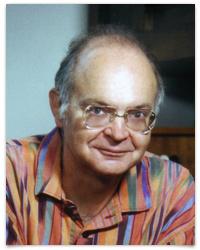
\includegraphics[scale=.5]{images/don_knuth.jpg}
\end{center}
	\caption{Don Knuth, the inventor of \TeX}
	\label{fig:sample}
\end{figure}

\section{Basic Terminology}
As usual the very basic terminology is briefly explained here. Most probably the explanations here only scratch a surface level. More detailed explanations of terminology goes into chapter~\ref{cha:theoretical-background}.

\section{Related Work and Projects}
Here a survey of other work in and around the area of the thesis is given. The reader shall see that the authors of the thesis know their field well and understand the developments there. Furthermore here is a good place to show what relevance the thesis in its field has.

\section{Structure of the Thesis}
%dsflkjas flaksjfl asdfj as lfjldsajflaksdjf sa dfjlasdkfj sadlfjasdklf als dfj l dfsdfsdfn chapter~\ref{cha:used-technologies} (\nameref{cha:used-technologies}) on page~\pageref{cha:used-technologies} we describe the used technologies.
Finally the reader is given a brief description what (s)he can expect in the thesis. Each chapter is introduced with a paragraph roughly describing its content.
\chapter{XIBO-Server}
\section{Beschreibung}
Als zentrale Steuereinheit wird ein XIBO-Server verwendet. Um diesen verwenden zu können, war es Notwendig sich in die Dokumentation einzulesen und die API-Schnittstelle auszuprobieren. Die Website des Servers diente vorerst als Übungsumgebung dadurch wurde es leicht auch die einzelnen Funktionen, inklusive der Vorgangsweise, des Servers zu verstehen.

\section{API-Schnittstelle}
Die API-Schnittstelle des XIBO-Servers ist mittels Swagger Dokumentiert, diese Dokumentation deckt die Grundfunktionalitäten und die Form der Anfragen ab. Da die Schnittstelle des Servers später als wesentliches Verbindungsstück zwischen der eigens entwickelten Steuerungssoftware und dem Server dient war es Nötig diese gründlich zu Testen und diese auch zu verstehen. Anfangs wurde dafür mit Postman gearbeitet. 


\section{Authentifizierung}
Es stellte sich heraus, dass die Authentifizierung mittels OAuth2 sehr speziell war was zu Beginn zu einigen Schwierigkeiten führte, da es einige Anläufe brauchte um herauszufinden wie die Parameter übergeben werden müssen und in welcher Reihenfolge. Dazu wurde eine Java-Klasse entwickelt welche die Authentifizierung automatisch übernimmt.
VERWEIS!!!!!!!!!!!!!!!!!!
https://oauth.net/2/

Der Server benötigt zur Authentifizierung mit einem Client eine Client_ID diese wird vom Server für jeden Client eindeutig erzeugt. Man bekommt sie direkt von der Website des Servers. 
Weiteres wird ein Client_Secret benötigt welches ebenso wie die Client_ID vom Server,für jede Anwendung ,eindeutig erzeugt wird und auch auf der Website erhältlich ist. Zudem ist ein Parameter in der Form "&grant_type=client_credentials" mitzugeben.

Zuerst wird ein Request-Body erstellt dieser hat folgende Parameter in der Form: 
 "client_id=<CLIENT_ID>&client_secret=<CLIENT_SECRET>&grant_type=client_credentials"
,die im Body mitgegeben werden und als Format "application/x-www-form-urlencoded"  haben. Anschließend werden dem Header noch der "content-type" mit dem Wert "application/x-www-form-urlencoded" und der Parameter "cache-control" mit dem Wert "no-cache" hinzugefügt. Als ergebniss der Anfrage bekommt der Client einen "access_token", dieser ist nun bei jeder Anfrage von Nöten um sich beim Server zu authentifizieren und es dem Client zu ermöglichen Daten abzurufen beziehungsweise weiterzugeben.

\section{Request-Helper}
Um in weiterer folge die Anfragen an den Digital Signage Server einfach und einheitlich durchzuführen gibt es die Klasse "RequestHelper". In dieser Klasse gibt es neben den beiden Parametern "responseBody" und "responseCode", welche zur Fehlerausgabe und zum Erhalt der Daten aus der Anfrage vorhanden sind, auch noch die Methode "executeRequest", diese übernimmt die Hauptaufgabe der Klasse und führt die Anfragen an das Signage System durch.

Die Parameter dieser Methode Lauten wie folgt:

\begin{itemize}
	\item {\em RequestTypeEnum:} Der Parameter vom Typ Enum wird genutzt um Herauszufinden welche Http Anfrage vorliegt. Mögliche Werte sind hierbei GET, POST, PUT und DELETE.
	
	\item {\em Params:} Hier liegt eine HashMap vor, die als Key-Value Paare alle Benötigten Parameter für den RequestBody beinhaltet. Beispielsweise: "LayoutID":"78", hierbei ist "LayoutID" der Key und "78" das Value.
		
	\item {\em Url:} Beinhaltet die URL unter der die Anfrage erreichbar ist. 
	
	\item {\em Token:} Ist jener Parameter der den "access_token",der benötigt wird um sich beim Server zu authentifizieren. Der Erhalt dieses Parameters, funktioniert wie bereits im vorigen Unterpunkt Authentifizierung beschrieben.
	
\end{itemize}

Zu beginn der Methode wird anhand des Parameters RequestTypeEnum unterschieden, um welche Http Anfrage es sich handelt. Wird GET oder DELETE geliefert wird durch die HashMap iteriert und die einzelnen Key-Value Paare als QeryParameter in der URL einfügt. Beispielsweise: <URL>/layout?layoutID=78&token=ajdlfjßßwkflkd6545.
Handelt es sich um eine POST oder PUT Anfrage so werden die Key-Value Paare im Body mitgegeben und im Format "application/x-www-form-urlencoded" codiert. Anschließend wird noch die URL mittels HttpUrl.Builder erstellt und ausgegeben. 




Als Ergebnis der Anfrage, mit den Parametern, in der Form
----------STütz fragen ob bsp für request usw einbauen




% create further tex files for all other chapters of your document
\chapter{Summary}
Here you give a summary of your results and experiences. You can add also some design alternatives you considered, but kicked out later. Furthermore you might have some ideas how to drive the work you accomplished in further directions.



\bibliography{da_bibliography}{}
\bibliographystyle{alphaurl} % save alternatives are abbrvurl	alphaurl	plainurl	unsrturl

\listoffigures
\listoftables
\chapter*{Project Log Book}
\begin{tabular}{|l|l|l|l|}
\hline
Date & Participants & Todos & Due\\
\hline
\end{tabular}

\appendix
\chapter{Additional Information} \label{cha:additional-information}
If needed the appendix is the place where additional information concerning your thesis goes. Examples could be:
\begin{itemize}
	\item Source Code
	\item Test Protocols
	\item Project Proposal
	\item Project Plan
	\item Individual Goals
	\item \ldots
\end{itemize}
Again this has to be aligned with the supervisor.
\chapter{Individual Goals} \label{cha:individual-goals}
This is just another example to show what content could go into the appendix.
\end{document}  